\chapter{Multi-Modeling in MATSim: PSim}
\label{ch:psim}
% ##################################################################################################################

\hfill \textbf{Author:} Pieter Fourie

\begin{center} 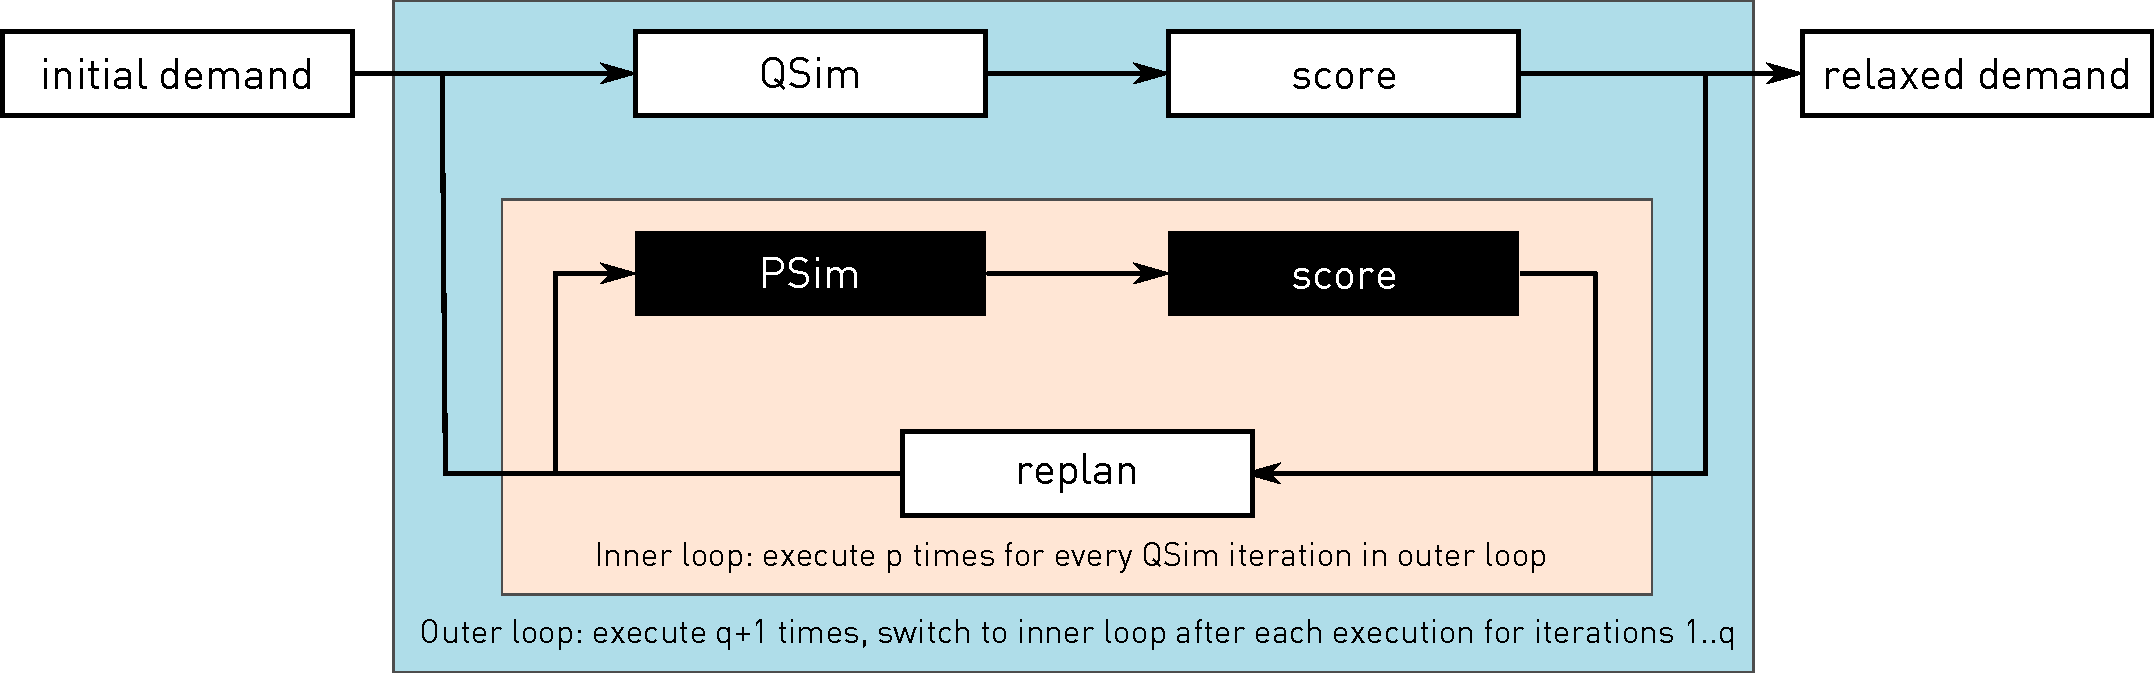
\includegraphics[width=0.5\textwidth, angle=0]{extending/figures/PSim/psim.pdf} \end{center}

\editdone{This text has undergone the professional edit. Please no grammatical changes anymore! They are most-probably wrong.}

\createStandardInformation{todo}{todo}{todo}{\citet[][]{FourieEtAl_TRR_2013}}

% ##################################################################################################################
\section{Introduction}
\gls{matsim}'s major current performance limitation is the network loading simulation, \ie the \gls{mobsim}, for example \gls{qsim} or \gls{jdeqsim}; 
this chapter focuses on \gls{qsim}. 
As shown earlier, \gls{qsim} is repeatedly executed in the \gls{matsim} loop for the entire agent population (Section~\ref{sec:inbrief}).

With the multi-modeling approach \citep[][]{FourieEtAl_TRR_2013}, shown in Figure~\ref{fig:PSim}, a \gls{matsim} run periodically replaces \gls{qsim} for a number of iterations with a simplified meta-model or \gls{psim}, running approximately one hundred times faster. 
In risk analysis, these models are called ``surrogate models'' \citep[][]{Sudret_APSSRA_2012}. 
\gls{psim} uses travel time information from the preceding \gls{qsim} iteration to estimate how well an agent day plan might perform, allowing multiple iterations of mutation and evaluation between \gls{qsim} iterations to more rapidly explore the agents' solution space, producing better performing plans in a shorter time.

% ------------
\createfigure%
{Operation of a \protect\gls{matsim} run implementing pseudo-simulation}%
{Operation of a \protect\gls{matsim} run implementing pseudo-simulation}%
{\label{fig:PSim}}%
{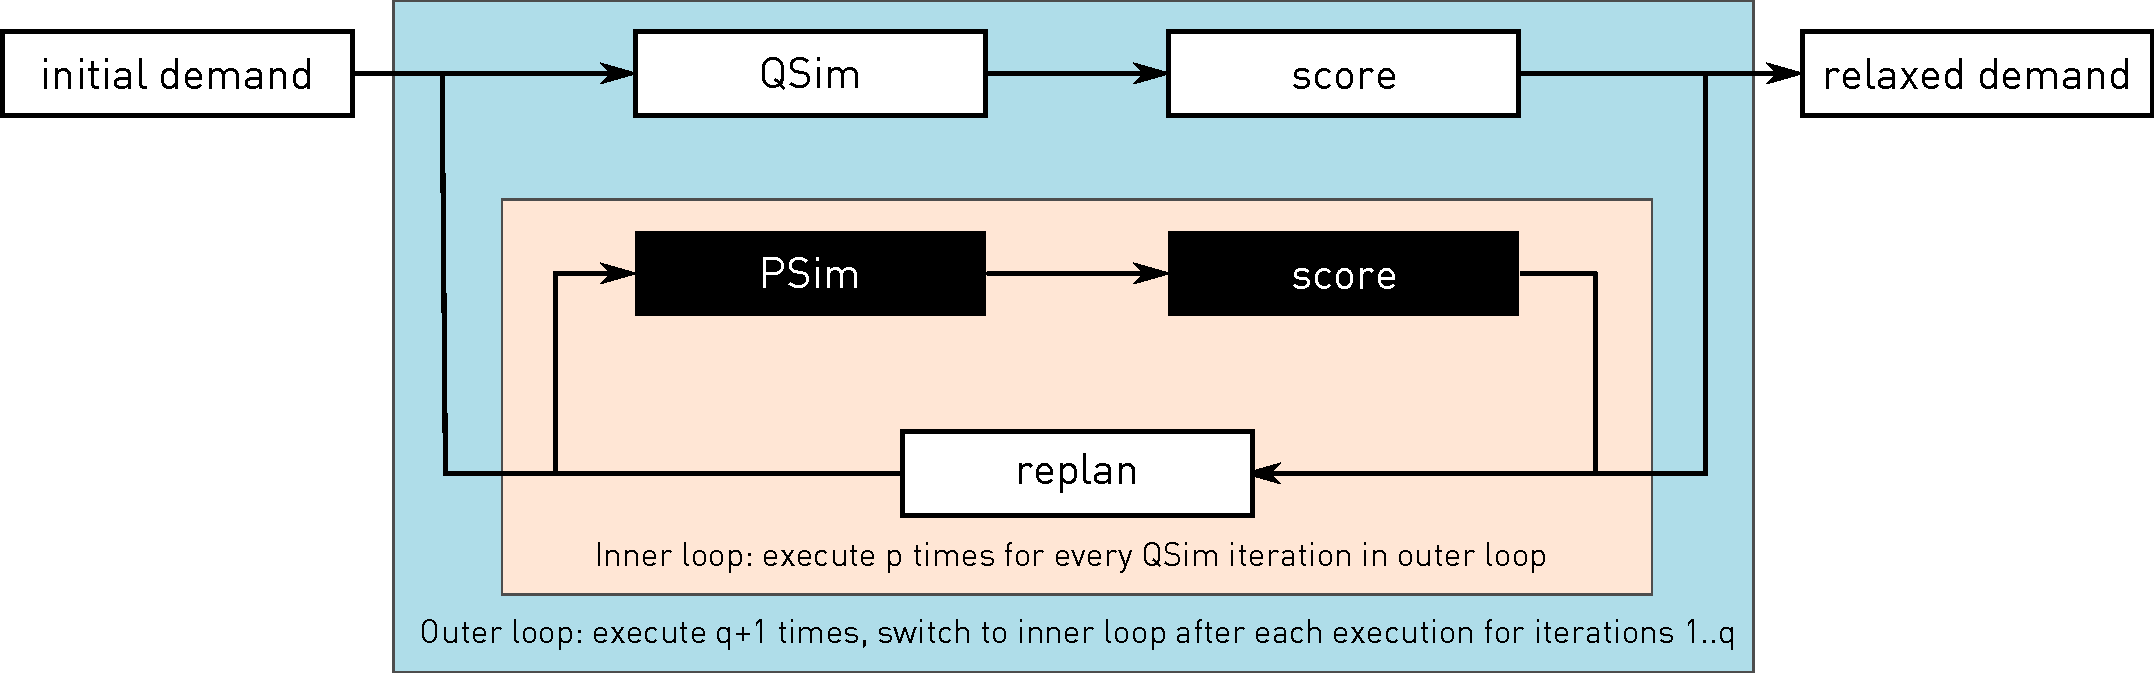
\includegraphics[width=0.7\textwidth, angle=0]{extending/figures/PSim/psim.pdf}}%
{}
% ------------

% ##################################################################################################################
\section{Basic Idea}
\gls{psim} exploits classes that record various network performance aspects during queue simulations and uses them as an approximate meta-model of \gls{qsim}. It fires the same sequence of events for car and public transport passengers that is produced during a \gls{qsim} mobility simulation, except that event timings are approximate values expected at the time of day they occur.

For private vehicle traffic, it calls the \lstinline|getLinkTravelTime(Link link, double time, Person person, Vehicle vehicle)| method of classes implementing the \lstinline|TravelTime| interface to fire \lstinline|LinkEnterEvents| and \lstinline|LinkLeaveEvents| at appropriate times for all car route links. For public transportation, the events sequence generated for a passenger traveling on a particular service relies on a meta-model of stop-to-stop travel times (\lstinline|interface StopStopTime|) and waiting times at stops (\lstinline|interface WaitTime|); both concepts were developed by Sergio Ord\`o\~nez at the Future Cities Laboratory (package \lstinline|playground.singapore.transitRouterEventsBased|).

\gls{psim} plans are scored using the same function as  \gls{qsim} iterations and are compatible with most replanning modules in \gls{matsim}. Following a series of \gls{psim} iterations, a plan is selected for each agent, in the usual fashion, and a \gls{qsim} iteration is run to start a new cycle. The various classes used in \gls{psim} are updated with the latest network performance information and the process repeats.

% ##################################################################################################################
\section{Performance}
Initial tests on the Zürich scenario (described in Chapter~\ref{ch:zhscenario}) have shown a dramatic decrease in computation times, compared to the default \gls{qsim}-only approach; performance improves linearly with an increasing number of computational cores.
Figure \ref{fig:PSimPerformance} compares the \gls{psim}-approach, in two configurations, against the existing approach, for a 10\,\% sample of private vehicle traffic in Zürich. All simulations were run until they reached a target score, \ie the score reached after running the standard approach for 100\,iterations. The first \gls{psim}-implementing configuration uses the same rate of plan mutation as the \gls{qsim}-only approach, where 30\,\% of agents are selected for plan mutation (replanning) after each iteration, whether it is a \gls{qsim} or \gls{psim} iteration. The new approach requires fewer \gls{qsim} iterations to reach a target score, but requires more time for replanning. Replanning is fully multi-threaded, with no synchronization between cores required, so its performance increases linearly, with increasing number of cores; times improve more dramatically with the new approach than the standard approach.
In the second configuration, the mutation rate is reduced and the number of \gls{psim} iterations between \gls{qsim} iterations increased to 24 for each \gls{qsim} iteration. The system now tests many more combinations of different mutation operations (four in this case: activity timing, mode choice, secondary activity location choice, and re-routing), to reach the target state much faster, even though it produces a smaller expected number of mutated plans per agent between \gls{qsim} iterations (three for configuration~1, 2.5\,plans for configuration~2).

This last point raises an interesting issue; namely, that the distribution of mutation operation numbers can be dramatically spread out with the \gls{psim} approach, because increasing the number of iterations is relatively cheap. This should make the approach preferable, especially with random mutation-producing replanning strategies, where a large number of mutations are needed to produce a relaxed simulation state.

For a detailed discussion of the meta-modeling approach and the results of applying this method to the Zürich scenario, refer to \citet[][]{FourieEtAl_TRR_2013}.

% ------------
\createfigure%
{\protect\gls{psim} computation time}%
{Computation time contributions vs. number of computational cores for \protect\gls{qsim}-only (0.3\,replanning rate), 9\,\gls{psim} iterations per \gls{qsim} iteration at 0.3\,replanning rate, and 24\,\gls{psim} iterations per \protect\gls{qsim} iteration at~0.1\,replanning rate}%
{\label{fig:PSimPerformance}}%
{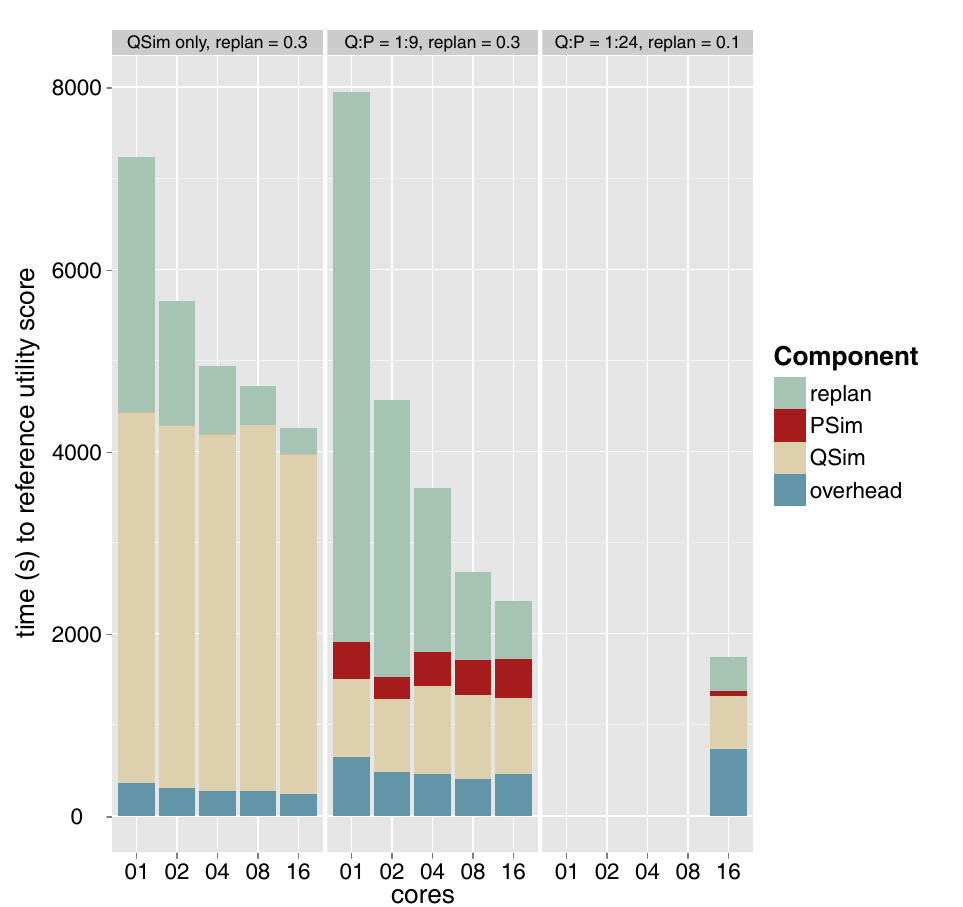
\includegraphics[width=0.7\textwidth, angle=0]{extending/figures/PSim/times}}%
{}
% ------------

% ============================================================================================
\subsection{Distributed Computing}
Because \gls{psim} executes plans independently from each other, requiring no coordination of computational processes, it is possible to distribute it across multiple nodes, with no need of shared memory, as illustrated in Figure~\ref{fig:distributedPSim}. To this end, we (Fourie and Ord\`o\~nez, \gls{fcl}) are implementing a simple messaging protocol to transmit network performance objects to \gls{psim} slave nodes from a master node running \gls{qsim} only. Slave nodes perform replanning operations and evaluate plans in a pre-determined number of \gls{psim} iterations per cycle. At the start of each \gls{qsim} iteration, a single plan for each agent is transmitted back to the master from all the slaves, and updated \lstinline|TravelTimes, StopStopTimes and WaitTimes| are rendered during the full mobility simulation, to be transmitted back to the slaves in the next cycle.

The approach yielded promising results, with a reduction in the number of \gls{qsim} iterations, as in the previous work, as well as the potential for running large-scale simulations on much cheaper hardware than the current approach, that demands expensive shared memory servers. Most importantly, all replanning takes place in parallel with the \gls{qsim} running on the master, so the time spent waiting for replanning operations can be reduced to nil. This performance increase is especially useful for large scenarios implementing public transportation, where the time spent replanning can be up to twice that of the queue simulation.

% ------------
\createfigure%
{Master-slave configuration for running PSim}%
{Master-slave configuration for running PSim in distributed mode, across many slave computer nodes in a local area network or in a cloud computational framework. The master runs selected plans in a full queue simulation and transmits updated travel time information to slave nodes after every iteration. In turn, slaves produce and evaluate new plans in repeated \gls{psim}/replanning cycles, sending the master a single plan for each agent at the start of a \protect\gls{qsim} iteration}%
{\label{fig:distributedPSim}}%
{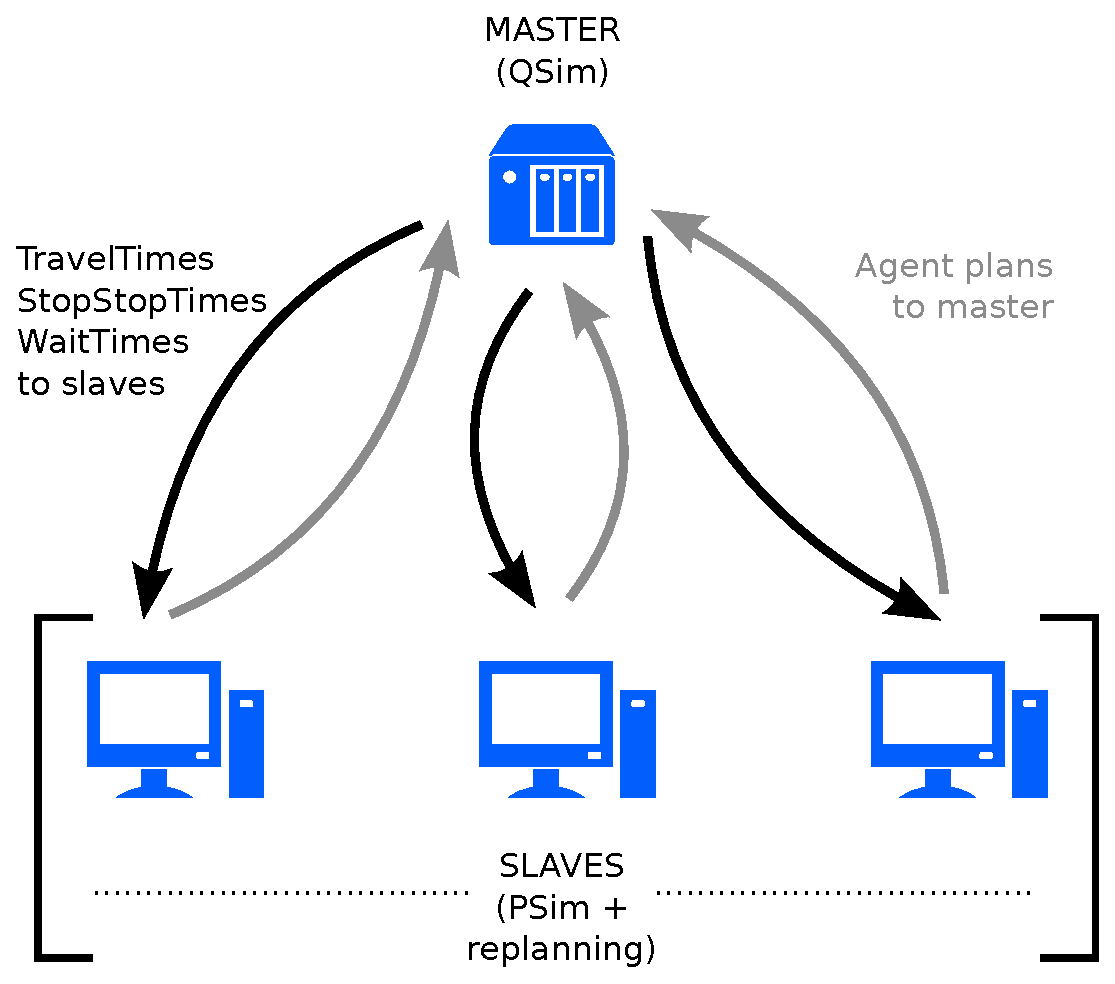
\includegraphics[width=0.7\textwidth, angle=0]{extending/figures/PSim/distributed}}%
{}
% ------------

% ##################################################################################################################
